\clearpage\begingroup\SourceLeaf{102b}\HistoricalHead{97}{R}{GAUSS AN GERLING UND OLBERS.}\HistoricalFoot{XI1.}{13}
\begin{center}[16.]\end{center}
\begin{center}\textsc{Gauss} an \textsc{Olbers}.\quad [Göttingen, Februar 1835\textsuperscript{*})].\end{center}
\begingroup\renewcommand{\thefootnote}{}
\footnotetext{[\textsuperscript{*}) Der Brief hat weder Unterschrift noch Zeitangabe.]}
\endgroup
\begin{center}\begin{minipage}{.88\linewidth}\centering\hrule\vspace{3pt}
\small [\textsc{Wilhelm Olbers}, Sein Leben und seine Werke, II, 2, S. 617.]
\par\vspace{3pt}\hrule\end{minipage}\end{center}
\noindent\hspace*{\parindent}.\ .\ .\ .\ .\ .\ .\ Ueber das, was seit Juli 1834 hier Neues hinzugekommen, werde
ich vielleicht bald eine Notiz in den G. A.\,[\textsuperscript{**}] geben.\begingroup\renewcommand{\thefootnote}{}
\footnotetext{[\textsuperscript{**}) Göttingische Gelehrte Anzeigen vom 7. März 1835, S. 345, Werke V, S. 528.]}
\endgroup\ Die 25pfündige Nadel in
der Sternwarte, mit ihrem Multiplicator von 270 Windungen unter 2700 Fuss
Drahtlänge, in der grossen bis zum phys. Cabinet gehenden Kette, worin der
Strom eine Drahtlänge von fast \(\frac{1}{2}\) Meile zu durchlaufen hat, bietet zu vielen
interessanten Versuchen Gelegenheit, die noch auf lange Zeit Beschäftigung
geben, und noch umfassendere geben könnten, wenn die Geldmittel nicht so
beschränkt wären! Ein Versuch gehört aber zu den schönsten, die in diesem
Fach je gemacht sind, und wird wohl den meisten Naturforschern sehr überraschend
sein, obwohl ich nicht durch Zufall, sondern durch Prämeditation
darauf gekommen bin und des Erfolgs schon gewiss war, noch ehe ich ihn
gemacht hatte. Es ist folgender:

Wenn die 25 {\fontspec{FreeSerif.otf}℔} Nadel in beträchtliche Schwingungen gesetzt wird, z. B.
so grosse, wie der Kasten verstattet, etwa \(27^0\), so können dabei die Nadeln im
\clearpage\SourceLeaf{103}\HistoricalHead{98}{L}{PHYSIK. BRIEFWECHSEL.}
\noindent m[agnetischen] O[bservatorium] und im phys. C[abinet] vollkommen in Ruhe sein
und bleiben darin, wenn die Kette nicht geschlossen ist oder eine der Nadeln
davon abgesperrt ist. Ist oder wird aber die Kette geschlossen, so dass die
Multiplicatoren im magn[etischen] Obs[ervatorium] und im Ph[ysicalischen]
C[abinet] mit darin sind, so fangen diese beiden Nadeln augenblicklich an
mitzuschwingen. Aber am merkwürdigsten ist die Art der Schwingungen.
Die natürliche Schwingungsdauer der Nadeln ist
\begin{center}\begin{tabular}{r@{\ }l@{\ }r}
25 {\fontspec{FreeSerif.otf}℔}&in der Sternwarte\quad .\quad .\quad .\quad .\quad .\quad .\quad .\quad .&\(42''{,}3\)\\
4 {\fontspec{FreeSerif.otf}℔}&im m[agnetischen] O[bservatorium]\ .\quad .\quad .&\(20{,}5\)\\
1 {\fontspec{FreeSerif.otf}℔}&im ph[ysikalischen] C[abinet]\quad .\quad .\quad .\quad .&\(13{,}8\)
\end{tabular}\end{center}
\noindent so dass z. B. für die Nadel im m[agnetischen] O[bservatorium] die Stellung auf
der Scale in jedem Augenblick \(t\) durch die Formel
\[
A+R\cos\left(\tfrac{t-T}{20''{,}5}\cdot180^0\right)
\]
\noindent ausgedrückt wird, wenn \(A\) die Stellung der Nadel in Ruhe, \(R\) die an sich
willkürliche halbe Schwingungsgrösse, \(T\) eine Epoche bedeutet, wo die Nadelstellung
im Maximum war. Allein wenn die sympathetischen Schwingungen
eintreten, so sind diese, allgemein zu reden, immer gemischte, nemlich eine
natürliche von willkürlicher und eine inducirte von bestimmter Grösse, z. B.
unter obigen Voraussetzungen die Formel
\[
A+R\cos\left(\tfrac{t-T}{20''{,}5}\cdot180^0\right)+r\cos\left(\tfrac{t-T'}{42''{,}3}\cdot180^0\right).
\]
\par\noindent\hspace*{\parindent}Dieses \(r\) ist dem Schwingungsbogen der grossen Nadel proportional und,
wenn dieser am grössten ist, etwa \(=20\) Scalentheile. Fast noch merkwürdiger
ist der a priori vorausgesehene und in der Erfahrung auf das Vollkommenste
bestätigte Umstand, dass die inducirten Schwingungen, welche mit
den inducirenden von gleicher Dauer sind, mit diesen nicht gleichen Anfang
haben, sondern eine halbe Schwingungsdauer (das Bogenargument \(90^0\)) davon
abstehen. Die gezeichneten Figuren sehen allerliebst aus, und ich habe es
in meiner Gewalt, das \(R\) oder die natürliche Schwingung unmerklich zu
machen, wo dann die Nadel also rein eine ihr nicht natürliche Schwingung
zu machen gezwungen ist; sobald die Kette geöffnet wird, nimmt die Nadel
sogleich wieder ihre natürliche Schwingung allein an.
\clearpage\SourceLeaf{104}\HistoricalHead{99}{R}{GAUSS AN OLBERS.}\HistoricalFoot{}{13\textsuperscript{*}}
\noindent\hspace*{\parindent}Ganz ähnliche Erscheinungen im phys. C[abinet], nur dass aus den Statt
habenden Grössenverhältnissen das \(r\) kleiner wird als im m[agnetischen] O[bservatorium].

Am allermerkwürdigsten aber ist der gleichfalls genau vorausgesehene
Fall, wo in der Kette eine zweite Nadel ist, deren natürliche Schwingungsdauer
der der grossen gleich ist. Ich hatte dies nicht sofort realisiren können,
aber jetzt ist dies auch geschehen, genau mit dem erwarteten Erfolg. Im
phys. C[abinet] wurde die Nadel, wie man es nennt, astatisch gemacht,
d. i. zwei Nadeln mit entgegengesetzten Polen verbunden, wovon die eine
etwas weniges stärker ist als die andere. Auf diese wirkt der
\par\noindent\begin{minipage}[t]{.78\linewidth}
Erdmagnetismus schwächer, daher längere Schwingungsdauer,
während der Multiplicator nicht bloss ebenso stark wie vorher,
sondern noch fast 50 p[ro]c[ent] stärker einwirkt. So wurde
die Schwingungsdauer dieser Doppelnadel auch genau auf \(42''{,}3\)
gebracht. Der Erfolg ist, dass für den Augenblick, wo die
Kette geschlossen wird, indem die 25 {\fontspec{FreeSerif.otf}℔}dige schon vorher
schwang, die im ph[ysikalischen] C[abinet] sofort auch anfängt
\end{minipage}\hfill\begin{minipage}[t]{.19\linewidth}\vspace{0pt}\centering
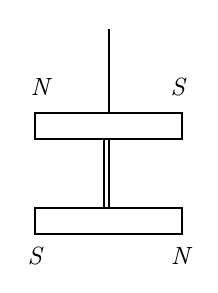
\begin{tikzpicture}[x=.0065in,y=-.0065in,line width=.65pt]
\draw (69,0)--(69,65);
\draw (12,65) rectangle (125,85);
\draw (65,85)--(65,138) (69,85)--(69,138);
\draw (12,138) rectangle (125,158);
\node[font=\small\itshape,inner sep=0pt] at (16,45) {N};
\node[font=\small\itshape,inner sep=0pt] at (122,45) {S};
\node[font=\small\itshape,inner sep=0pt] at (12,175) {S};
\node[font=\small\itshape,inner sep=0pt] at (124,175) {N};
\end{tikzpicture}\end{minipage}
\par\noindent zu schwingen, und diese Schwingungen, anfangs mässig, nahmen beständig an
Grösse zu, so dass sie nach \(\frac{1}{2}\) Stunde auf 300 angewachsen waren. Hier sind
nun aber die Elongationen mit denen der grossen Nadel \textls[120]{gleichzeitig}, obwohl
nach Lage der Umstände entweder gleichnamig (d. i. Maximum mit
Maximum) oder ungleichnamig (Maximum mit Minimum). Das ganze Phänomen
ist eine Art von Abspiegelung dessen, was im Sonnensystem vorgeht,
nämlich der periodischen Störungen im ersten Fall, der Säcularstörungen im
zweiten, nur haben sie den Vorzug, dass, während wir bei den Planetenstörungen
bloss müssige Zuschauer sind, wir hier die \textls[120]{eben so scharf} oder zum
Theil \textls[120]{noch viel schärfer} zu messenden Wirkungen selbst nach Gefallen
hervorbringen. Ueberhaupt ist die Schärfe in allen diesen Dingen bewundernswürdig.
Wir vergleichen z. B. durch derartige Manövers die Uhren in der
Sternwarte, dem m[agnetischen] O[bservatorium] und ph[ysicalischen] C[abinet]
jeden Augenblick auf \(0''{,}1\) genau, und ich bin vollkommen überzeugt, dass
wir auf dieselbe Art eben so sicher die Uhren in Göttingen und Bremen ohne
Zwischenstation direkt vergleichen könnten, wenn nur jemand das Geld dazu
hergeben wollte, eine \(\frac{1}{2}\) fingersdicke Kette von Kupferdraht von Göttingen
\clearpage\SourceLeaf{105a}\HistoricalHead{100}{L}{PHYSIK. BRIEFWECHSEL.}
\noindent nach Bremen zu führen. Vielleicht kann ich in Zukunft die Gleise von
Eisenbahnen zu analogen Zwecken benutzen.

Ich muss noch bemerken, dass freilich genau betrachtet, ebensogut die
Schwingungen der zweiten oder dritten Nadel, Schwingungen in den beiden
anderen erzeugen müssen; allein ich habe durch die Rechnung gefunden, dass
solche \textls[120]{unmerklich} sind, was auch die Versuche bestätigen. Vor der Hand,
d. i. so lange man sich nicht auch Nadeln von ähnlicher Kraft, wie meine
25 {\fontspec{FreeSerif.otf}℔}dige, oder stärkere verschafft, wird also dieser interessante Versuch der
sympathetischen Schwingungen in grosser Ferne anderwerts nicht nachgemacht
werden können. Ein paar solcher 25 {\fontspec{FreeSerif.otf}℔}diger Nadeln kommen übrigens
nach Copenhagen. Hier bleiben vorerst noch 12 oder 14. Eine etwas beträchtliche
Zahl muss man nothwendig besitzen, um in ihnen durch wiederholte
gegenseitige Verstärkung ihre volle Kraft hervorzurufen. \mbox{.\ .\ .\ .\ .\ .\ .\ .}
\clearpage\endgroup
